\documentclass[10pt]{book}

\usepackage[T1]{fontenc}
\usepackage{kpfonts}
\usepackage{amsmath}
\usepackage{amssymb}
\usepackage{amsthm}
\usepackage{mathtools}
\usepackage{empheq}
\usepackage{pgfplots}
\usepackage{cleveref}
\usepackage{graphicx}
\usepackage{geometry}
\usepackage{titlesec}
\usepackage{fancyhdr}
\usepackage{setspace}
\usepackage{microtype}
\usepackage{parskip}
\usepackage{tcolorbox}
\usepackage{booktabs}
\usepackage{float}
\usepackage{tikz}
\usepackage{wrapfig}

\geometry{a5paper, top=1.5cm, bottom=2cm, inner=1.8cm, outer=1.2cm}
\usetikzlibrary{arrows.meta, positioning, pgfplots.fillbetween}

\titleformat{\chapter}[display]{\normalfont\large\bfseries}{\chaptertitlename\ \thechapter}{10pt}{\large}
\titleformat{\section}{\normalfont\normalsize\bfseries}{\thesection}{1em}{}
\titleformat{\subsection}{\normalfont\small\bfseries}{\thesubsection}{1em}{}

\pgfplotsset{compat=1.18}

\title{Advanced Mathematics Applications}
\author{London Wallace}
\date{Semester 2, 2026}

\renewcommand{\chaptermark}[1]{\markboth{#1}{}}

\pagestyle{fancy}
\fancyhf{}
\fancyfoot[C]{\thepage}
\renewcommand{\headrulewidth}{0pt}
\fancypagestyle{plain}{\fancyhf{}\fancyfoot[C]{\thepage}\renewcommand{\headrulewidth}{0pt}}

\fancypagestyle{plain}{\fancyhf{}\renewcommand{\headrulewidth}{0pt}}

\setstretch{1.15}

\titlespacing{\chapter}{0pt}{-10pt}{10pt}

\newcommand{\newthought}[1]{\vspace{0.5\baselineskip}\noindent{\scshape #1}}

\renewcommand{\bibname}{Bibliography and Suggested Reading}

\begin{document}
\frontmatter
\maketitle
\tableofcontents

\chapter{Preface}
\newthought{These notes} follow the course \emph{Advanced Mathematics Applications},
taught by Lyle Noakes at the University of Western Australia in Semester 2 of 2026. The unit
teaches advanced techniques of calculus, including multivariable calculus, Green's, Stoke's and
divergence theorem, complex analysis, ordinary and partial differential equations, and
Sturm-Liouville theory.

\section{More detailed overview of the subject.}

\newthought{These notes} are about something but with more detail.

\section{Table of Symbols}
\begin{center}
  \begin{tabular}{cc}
    \toprule
    Symbol          & Meaning                       \\
    \midrule
    $\forall$       & For every \emph{or} for all   \\
    $\exists$       & There exists                  \\
    $ \in $         & In \emph{or} is an element of \\
    $ \subset $     & Is a proper subset of         \\
    $ \subseteq $   & Is a subset of                \\
    $ \cup $        & Union with                    \\
    $ \cap $        & Intersection of               \\
    $ \backslash$   & Not \emph{or} without         \\
    $ \varnothing $ & Empty set                     \\
    $ \sim  $       & Relates to                    \\
    $ > $           & Greater than                  \\
    $ < $           & Less than                     \\
    $ \ge $         & Greater than or equal to      \\
    $ \le $         & Less than or equal to         \\
    $|n|$           & The absolute value of $n$     \\
    $\qedsymbol $   & It has been proven            \\
    \bottomrule
  \end{tabular}
\end{center}
\mainmatter

\part{Essentials of Multivariable Calculus}
\chapter{Vectors, Vector Valued Functions, and Functions of Several Variables}
\section{The Vector Space $\mathbb{R}^n$}
\newthought{A vector space} $V$ on $\mathbb{F}$ is the set $V$ of objects named \emph{vectors} and a field\footnote{refer: Algebra}
$\mathbb{F}$ of objects name \emph{scalars}, with two operations \emph{vector addition} and \emph{scalar multiplication} defined:
\begin{enumerate}
  \item Vector Addition: $+$: $V \times V \to V$
  \item Scalar Multiplication: $\cdot$: $\mathbb{F} \times V \to V$
\end{enumerate}
That satisfies the axioms of a vector space. Namely that vector addition and scalar multiplication are both commutative, associative,
and distributive, and that there exists additive and multiplicative identities and inverses.

\newthought{The vector space $\mathbb{R}^n$} is the set $V = \{ (x_0, x_1, \ldots, x_n) : x_i \in \mathbb{R}\}$ over the real numbers.
Elements of $V$ are said to be $n$-tuples of real numbers. Vector addition is defined to be the coordinate-wise addition of elements
of $V$:
\[(x_0, x_1, \ldots, x_n) + (x'_0, x'_1, \ldots, x'_n) = (x_0 + x'_0, x_1 + x'_1, \ldots, x_n + x'_n)\]
with the usual arithmetic inherited from the real numbers. Scalar multiplication is defined as the distributive multiplication of each
coordinate by some $\alpha \in \mathbb{R}$:
\[\alpha \cdot (x_0, x_1, \ldots, x_n) = (\alpha \cdot x_0, \alpha \cdot x_1, \ldots, \alpha \cdot x_n)\]
In two and three dimensions, $n$-tuples of numbers can be thought of as a quantity with \emph{magnitude and direction}, and arrow
from the origin to $(x,y,z)$, however to not lose generality in higher dimensions it is best just to think of them as ordered lists of
real numbers, with arithmetic defined above.

\newthought{The dot product} of two vectors is defined:
\[\mathbf{a} \cdot \mathbf{b} = \sum_{n=1}^{n}a_ib_i\]
for two vectors $\mathbf{a}, \mathbf{b} \in \mathbb{R}^n$. An alternative formulation of the dot product is:
\[\mathbf{a} \cdot \mathbf{b} = \|\mathbf{a}\|\ \|\mathbf{b}\| \cos\theta\]
where $\theta$ is the angle between $\mathbf{a}$ and $\mathbf{b}$, and $\|\mathbf{a}\|$ is the magnitude, or length, of $\mathbf{a}$.
Thus, two orthogonal vectors will have a dot product of 0 (since $\cos(\pi / 2) = 0$) and two parallel vectors will have a dot product
equal to the product of their magnitudes. Notice
\[\mathbf{a} \cdot \mathbf{a} = \|\mathbf{a}\|^2 \implies \|\mathbf{a}\| = \sqrt{\mathbf{a} \cdot \mathbf{a}}\]
The dot product can be thought of geometrically as a measure of how much of $\mathbf{a}$ \emph{goes in} the direction of $\mathbf{b}$.
A handy application of this fact is determining the $x, y$, and $z$ components of a vector $\mathbf{a}$, by taking its dot product with
the standard basis vectors\footnote{\ $\mathbf{i} = (1,0,0),\ \mathbf{j} = (0,1,0),\ \mathbf{k} = (0,0,1)$} $\mathbf{i}, \mathbf{j}$, and
$\mathbf{k}$, respectively.

\begin{wrapfigure}{o}{0.4\textwidth}
  \centering
  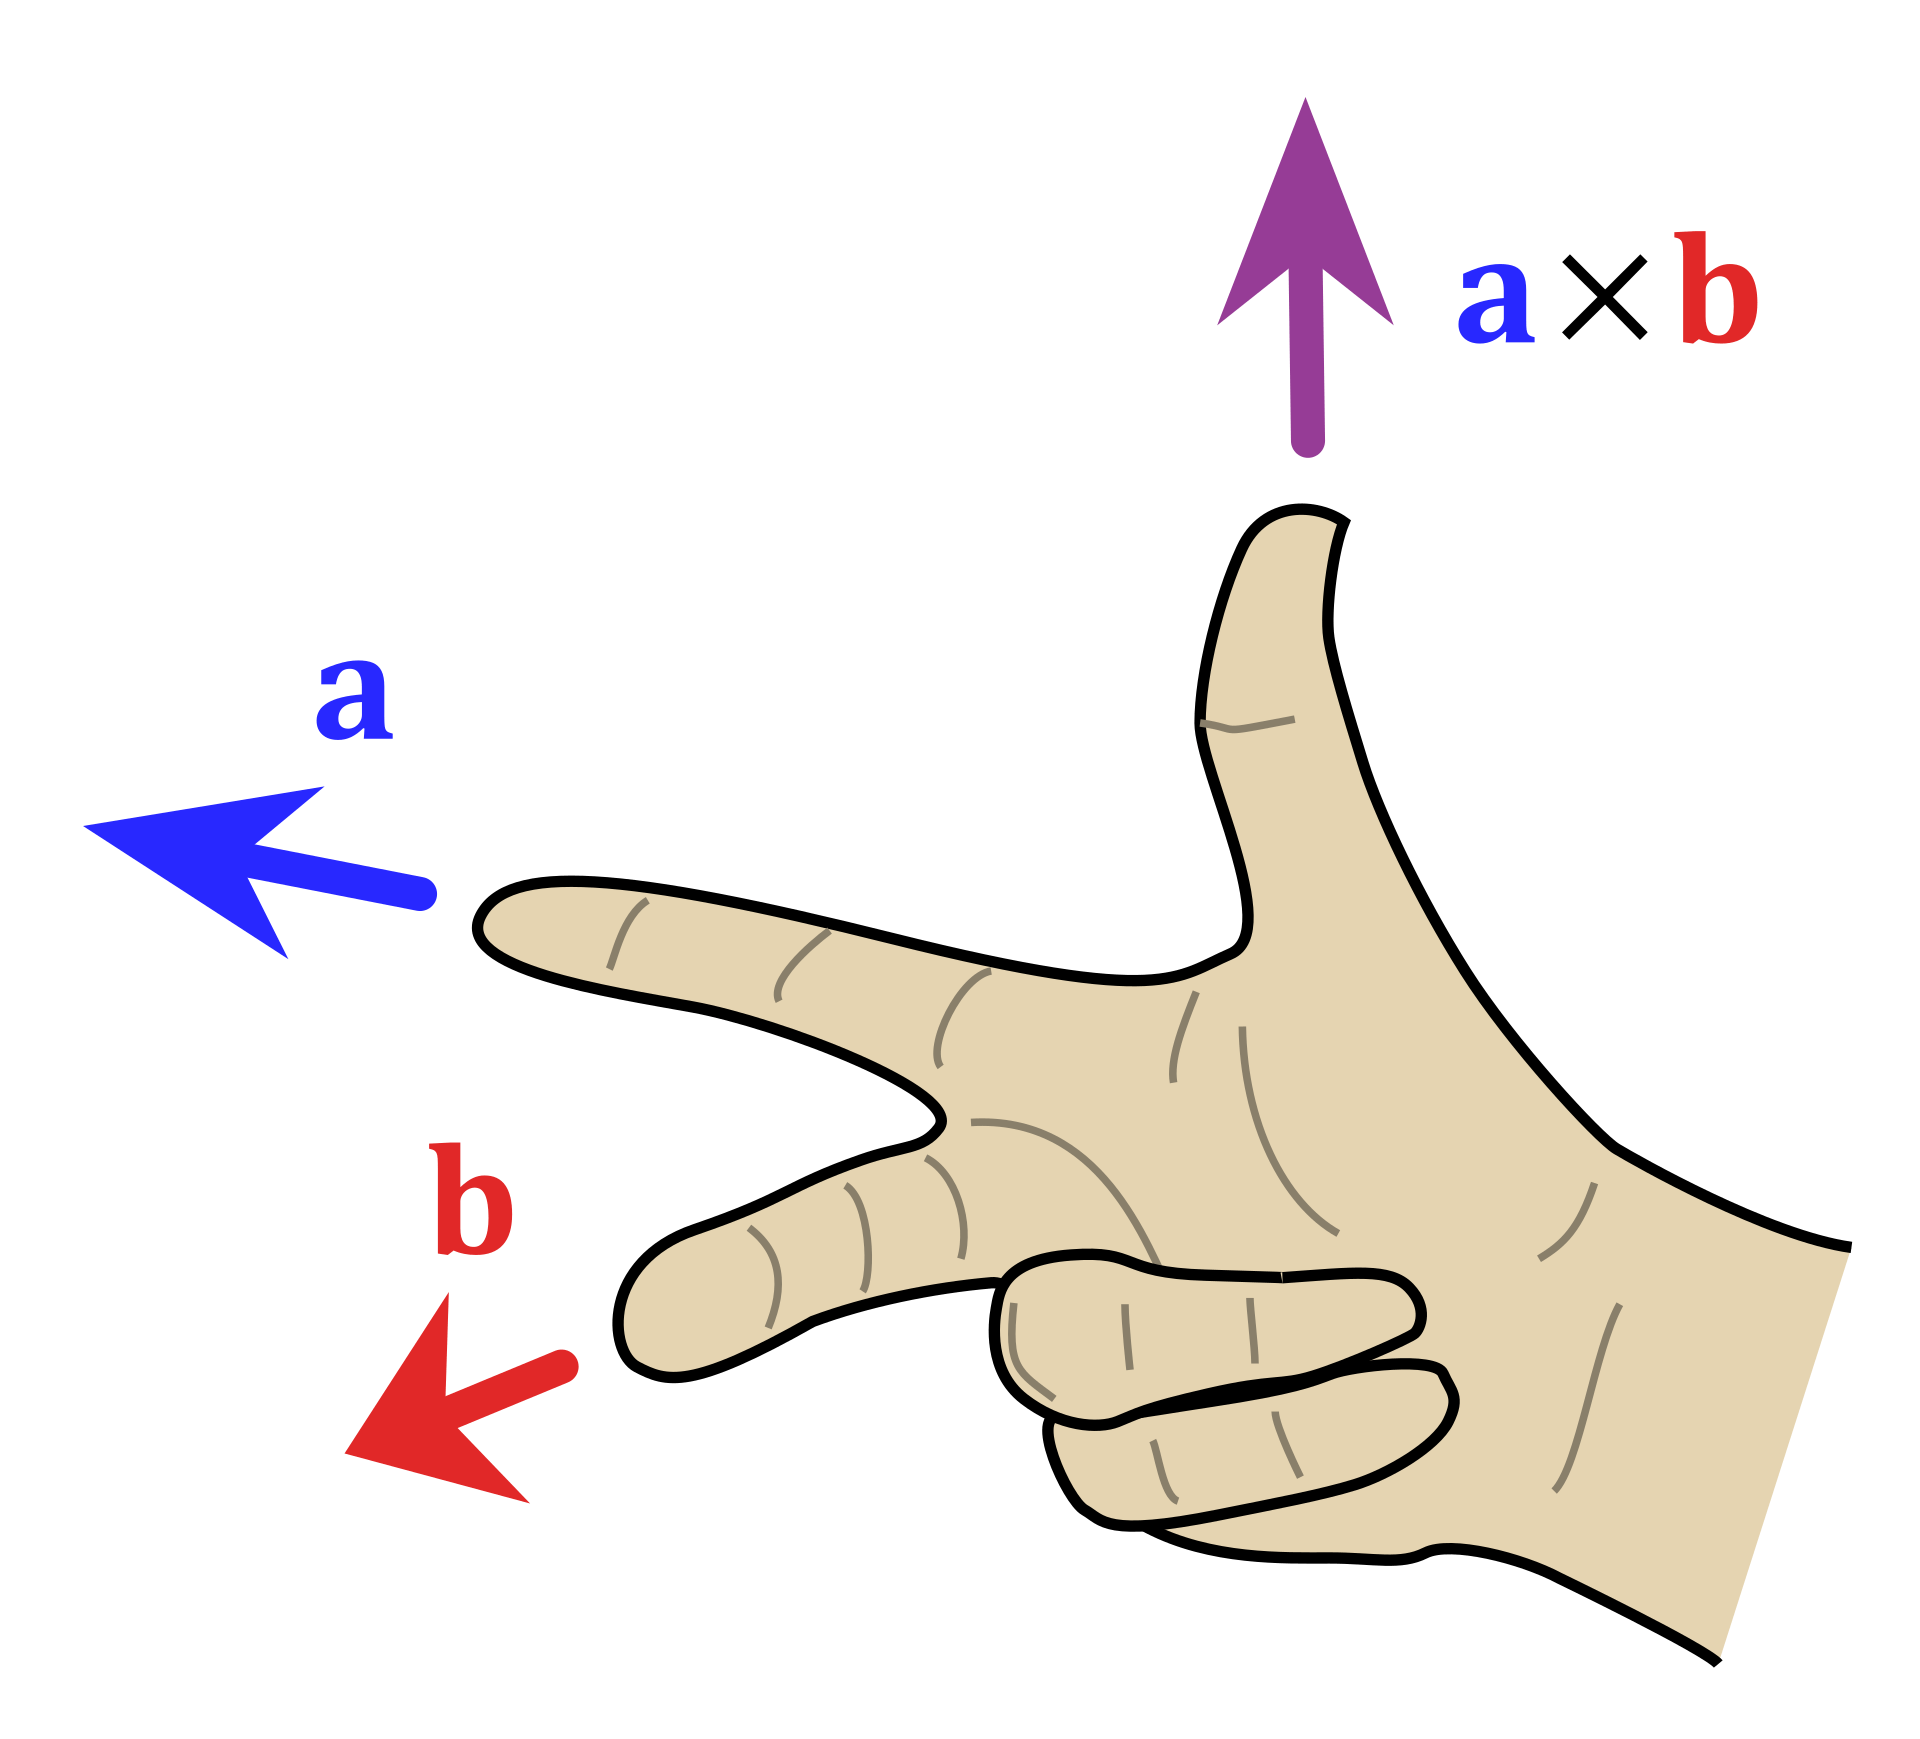
\includegraphics[width=0.38\textwidth]{right-hand-rule.png}
  \caption{The right hand rule is the convention used for the positive direction $\mathbf{n}$ in $\mathbf{a} \times \mathbf{b}$.}
  \label{fig:right-hand-rule}
\end{wrapfigure}

\newthought{The cross product} of two vectors $\mathbf{a}, \mathbf{b} \in \mathbb{R}^3$ is defined:
\[\mathbf{a} \times \mathbf{b} = (\|\mathbf{a}\|\ \|\mathbf{b}\| \sin\theta)\cdot \mathbf{n}\]
where $\theta$ is the angle between them and $\mathbf{n}$ is a unit vector perpendicular to the plane containing $\mathbf{a}$ and $\mathbf{b}$,
whose direction is given by the right hand rule (\cref{fig:right-hand-rule}). A vector perpendicular to a plane is said to be \emph{normal}
to that plane.

An easy way to calculate the cross product is to build the $3 \times 3$ matrix with first row $[\mathbf{i}\ \mathbf{j}\ \mathbf{k}]$,
second row $[\mathbf{a}]$, and third row $[\mathbf{b}]$, and take it's determinant.

\[
  \mathbf{a} \times \mathbf{b} =
  \begin{vmatrix}
    \mathbf{i} & \mathbf{j} & \mathbf{k} \\
    a_1 & a_2 & a_3 \\
    b_1 & b_2 & b_3
  \end{vmatrix}
\]
\[
  \mathbf{a} \times \mathbf{b} = (a_2b_3 - a_3b_2)\mathbf{i} + (a_3b_1 - a_1b_3)\mathbf{j} + (a_1b_2 - a_2b_1)\mathbf{k}
\]
Once you know a normal vector to a plane (usually by taking the cross product of two vectors in that plane) and one point in the plane,
it is easy to determine an equation for that plane, since the dot product of \emph{any} vector in the plane with the normal vector will be 0.
\[\mathbf{n} \cdot (x,y,z) = n_xx + n_yy + n_zz + d = 0\]
Simply plug in the $(x,y,z)$ that you know to determine the correct value of $d$.

\section{Vector Valued Functions}
\newthought{A function} $f$ is said to \emph{vector valued} if it is a mapping $\mathbb{R} \to \mathbb{R}^n$. In other words, vector valued
function take a real number and assign a vector.
\[\mathbf{r}(t) = (x_1(t), x_2(t), \ldots, x_n(t))\]
The functions $x_1(t), \ldots, x_n(t)$ are called the \emph{coordinate functions} of $\mathbf{r}$.

A common example of a vector valued
function is $\mathbf{r}(t)=(t,f(t))$ where $f:\mathbb{R} \to \mathbb{R}$ and $t\in[a,b] : a,b\in\mathbb{R}$. This function describes a
\emph{parametrisation} of $f$ and points from the origin to every point of $f$ as $t$ varies in its domain, as if the tip were moving
along $f$. It is helpful to imagine $t$ as representing time. This will be covered in more detail in Chapter 7.

\section{Functions of Several Variables}
\newthought{A function} $f$ is a \emph{multivariable} function if it is a mapping from $\mathbb{R}^n \to \mathbb{R}$. These functions take a
vector and assign to it a real number. The coordinates of the input vector can be thought of as several independent variables.
\[f(x_1,x_2,\ldots,x_n) = n\]
where $n$ is some combination of the variables $x_1, \ldots, x_n$. Just like we can plot a function of one variable $f: D \to R$ by defining
the line
$l = \{(x,f(x)) : x \in D\}$
as the set of all points that satisfy $(x,f(x))$, we can define an $n+1$ dimensional surface of a function
$f: D \subseteq \mathbb{R}^n \to R \subseteq \mathbb{R}$ of $n$ variables by
\[S = \{(x_1,x_2,\ldots,x_n,f(x_1,x_2,\ldots,x_n)) : x_1, \ldots, x_n \in D\}\]
Allowing an $n+1$ dimensional alien to understand its plot. The only application where this is useful to humans is to plot $z = f(x,y)$ In
three dimensions.

\newthought{Fields} are mappings $\mathbb{R}^n \to \mathbb{R}^m$, usually $\mathbb{R}^3 \to \mathbb{R}^m$. They can be thought of as
assigning to every point in space a vector in $\mathbb{R}^m$. A common example is a force or electromagnetic field. A scalar field is a
special multivariable function of three variables that assigns to every point in space a number, like temperature or pressure. These are
covered in Chapter 8.

\chapter{Limits and Continuity}
\chapter{Derivatives}
\chapter{Applications of the Derivative}
\chapter{The Riemann Integral}
\chapter{Double and Triple Integrals}
\chapter{Path and Surface Integrals}
\chapter{Vector Fields}

\end{document}